\large
\section{Code Explanation}

In this chapter, we will explain the implemented code by which the project is done. In this project, we classified the coding files into two section … the first one is the one that cares about the HTTP server and how it interact with the user and with the motor, the second section that cares about the programming of the RaspberryPi and the motor.


\subsection{HTTP Server}

In this section talking about the programming code by “JAVA” Programming Language of the HTTP Server. This Section contains one file which is the named file called “HTTP-Server”. But Before Explain the code … we must know the importance of the server in our project. It’s simply to send to the RaspberryPi (C++) Code a request with direction of the movement the user wants to move the body. If the user gives an order, the server replies with that order. It makes that cycle 10 times per one Second. It means that the user has the chance to give an order ten times in every second by any movement as Left, Right, Forward, Backward or stop from movement; so the (C++) code send a request for the server to give it any order and the reply of the java code includes the order of the movement.


\newpage
At the First of the java code … we start to import some java files that we will use indeed in the code.

\begin{figure}[h]
    \centering
\begin{tabular}{|c|c|}
    \hline
    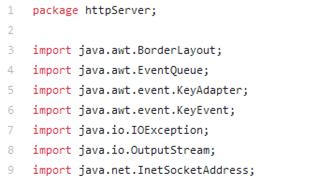
\includegraphics[width=.6\textwidth]{figures/42.1.png} & 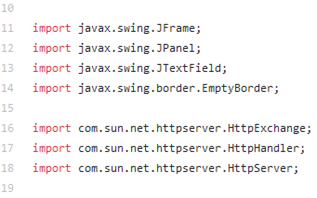
\includegraphics[width=.6\textwidth]{figures/42.2.png}\\
    \hline
\end{tabular}
    \caption{Java code: import section}
    \label{fig:my_label}
\end{figure}


At First we declared two variables that we will be used later in the java code … those variables are a Text field named text1 and the other one is a Panel named contentPane.  After that we create a new object from HTTP-Server class called frame and make it as visible. In this object we just call HTTP-Server Function that will be explained later in this code.

\begin{figure}[h]
    \centering
    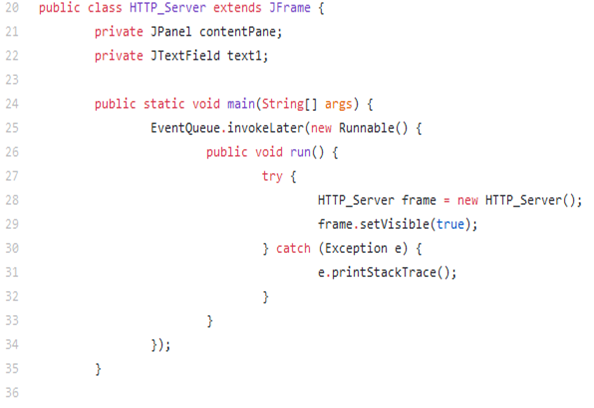
\includegraphics[width=.9\textwidth]{figures/43.png}
    \caption{Java code: Create new HTTP-Server}
    \label{fig:my_label}
\end{figure}

\newpage
Then, we have defined HTTP-Server function. This function makes a frame that Exit on Close and set some properties for it including the bounds. After that, make a new panel named content Pane with setting some properties to it including border and layout. Later, make a variable named server from HTTP-Server Type.

\begin{figure}[h]
    \centering
    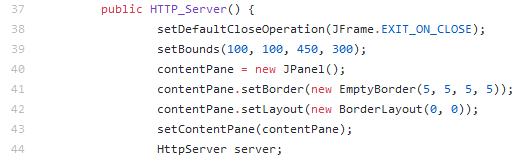
\includegraphics{figures/44.png}
    \caption{Java code: HTTP-Server Function}
    \label{fig:my_label}
\end{figure}

Simply, Here If everything is gone very well … Then we just create a default executor and start the server. On the other hand, if there is any error expected happened … Then Show Error Message.

\begin{figure}[h]
    \centering
    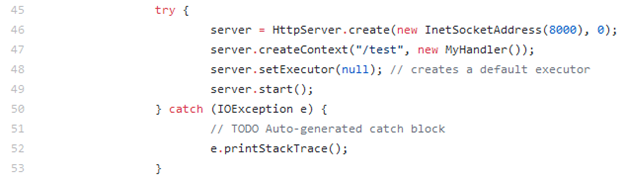
\includegraphics[width=1\textwidth]{figures/45.png}
    \caption{Java code: Server Start}
    \label{fig:my_label}
\end{figure}

\newpage

Later, We make textbox called text1 and set in it a text by “STOP” while customization of some of its properties like add it at the center of the content Pane and make it focus.

\begin{figure}[h]
    \centering
    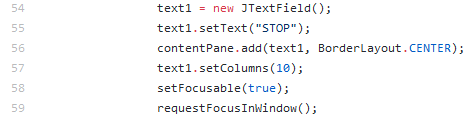
\includegraphics{figures/46.png}
    \caption{Java code: Textbox Creation}
    \label{fig:my_label}
\end{figure}

In this code we make a Listener for the key entry on which if the user pressed or typed by any Button … it save the key. While if the key is released then don’t save it.

\begin{figure}[h]
    \centering
    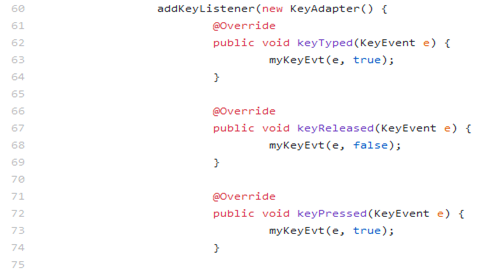
\includegraphics{figures/47.png}
    \caption{Java code: Key Listener}
    \label{fig:my_label}
\end{figure}

\newpage
Here we make some condition for the order … if the user press or type on the UP keyboard button then set text for text1 textbox as “UP”, While if the user press or type on the DOWN keyboard button then set text for text1 textbox as “DOWN”, While if the user press or type on the LEFT keyboard button then set text for text1 textbox as “LEFT”, While if the user press or type on the RIGHT keyboard button then set text for text1 textbox as “RIGHT” Or if nothing of these happened … then set text for text1 textbox as “STOP”.

\begin{figure}[h]
    \centering
    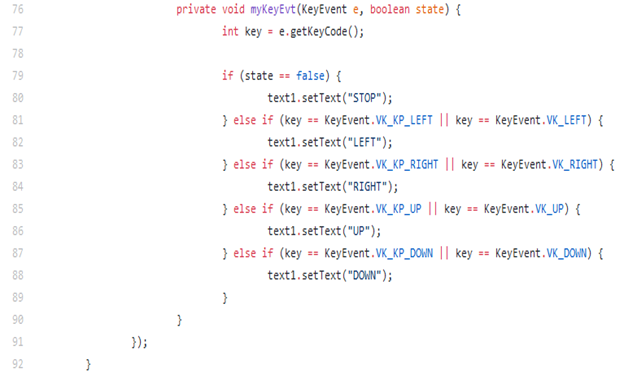
\includegraphics[width=.9\textwidth]{figures/48.png}
    \caption{Java code: response status code}
    \label{fig:my_label}
\end{figure}

\newpage

Finally, here when C++ code request an order … just get the order from the text1 text box and send the text as a reply for the code.

\begin{figure}[h]
    \centering
    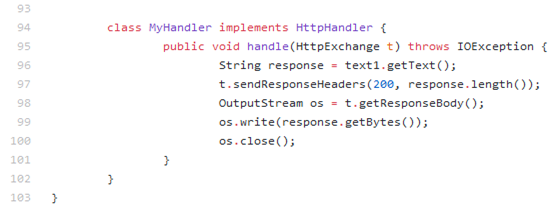
\includegraphics{figures/49.png}
    \caption{Java code: send reply}
    \label{fig:my_label}
\end{figure}

\newpage

\subsection{RaspberryPi}

In this section talking about the programming code by “C++” Programming Language of the RaspberryPi module and the motor. This Section contains three files which are the Motor header file, the Motor Function description file and finally and absolutely the Main project file. But Before Explain the code … we must shout out that we used a method in code called Pulse-width modulation (PWM) so we must have an small brief on the PWM and its principles in order to understand the way of design is made and has been coded by.

\subsubsection{Pulse-width modulation (PWM)}

Pulse-width modulation (PWM) is a strategy to reduce an electrical signal's average power by essentially cutting it into discrete sections. The average voltage (and current) value fed to the load is managed by switching the switch among both supply and load on and off at a quick rate. Compared to the off periods the longer the switch is on, the higher the total power supplied to the fee. Along with maximum power point tracking (MPPT), it is one of the primary ways of reducing solar panel output to that which a battery can use. PWM is especially suitable for running inertial loads such as motors which are not as easily influenced by this discrete switching because they have inertia for slow reaction. The frequency of PWM switching must be high enough not to affect the load, which is to say the resulting waveform perceived by the load must be as smooth as possible.

\begin{figure}[h]
    \centering
    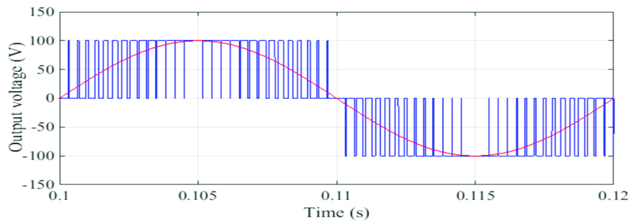
\includegraphics[width=.8\textwidth]{figures/50.png}
    \caption{Ideal pulse-width modulation (PWM)}
    \label{fig:my_label}
\end{figure}

\newpage

Depending on load and application, the rate (or frequency) at which the power supply has to switch can vary considerably. The main advantage of PWM is that it has very low power loss in the switching devices. There is virtually no current when a switch is off, and when it is on and power is transferred to the charge, there is almost no drop in voltage across the switch. Consequently, power loss, being the product of voltage and current, is close to zero in both cases. PWM also works well with digital controls which can easily set the required duty cycle because of their on / off nature.

\newpage
\subsubsection{Motor header code}

This code file named “motor.h” and it is responsible for the declaration of the function used in the main code. In the first, we made class by ‘Motor’ name that we can take object from it anytime we needed to. Any Class consists of public and private sections … For the public one, we declare function for motion which are forward, backward, turn Right, turn Left and stop. All those function doesn’t take or return any attribute. At last, in the public section, we also declare a function called ‘motor’ that takes six attributes which are pwmRightPin1, pwmRightPin2 those are the number of the Pulse Width Modulation Pin for the right side of the motor, pwmLeftPin1, pwmLeftPin2 those are the number of the Pulse Width Modulation Pin for the left side of the motor, pwmMinVal, pwmMaxVal those are the number of the Pulse Width Modulation value of the motor … all those attributes are from integer data type.
\newline
\begin{figure}[!h]
    \centering
    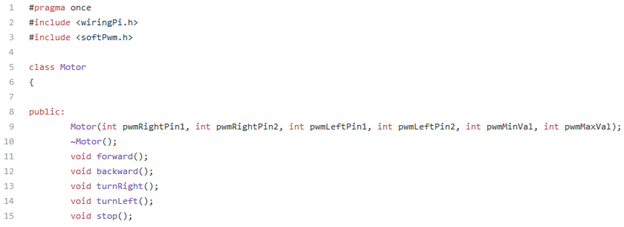
\includegraphics{figures/51.png}
    \caption{Motor header code: Public section}
    \label{fig:my_label}
\end{figure}

\newpage
After Public section, it is the turn for the private one … we declare function for motion which are left Side Forward, left Side Backward, right Side Forward, right Side Backward, left Side Stop and right Side Stop. Also we have declared a function called ‘init’ for initialization of the motor.  All those function doesn’t take or return any attribute as those in the public section. We also declare some variables for the Pulse Width Modulation which are pwmRightPin1, pwmRightPin2 … those are for the number of the Pulse Width Modulation Pin for the right side of the motor, pwmLeftPin1, pwmLeftPin2 … those are for the number of the Pulse Width Modulation Pin for the left side of the motor, pwmMinVal and pwmMaxVal … those are the number of the Pulse Width Modulation value of the motor. All those variables are from integer data type.

\begin{figure}[h]
    \centering
    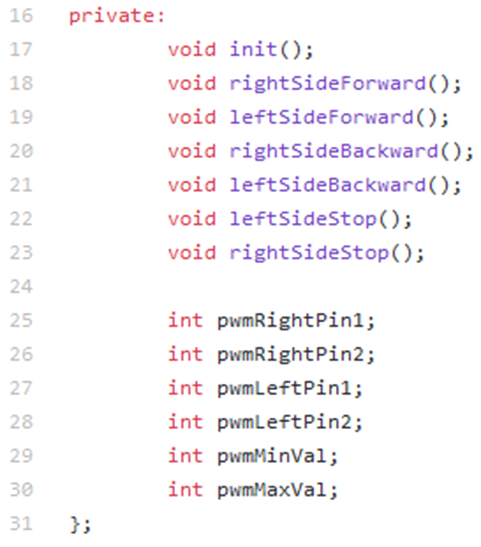
\includegraphics[width=.7\textwidth]{figures/52.png}
    \caption{Motor header code: Private section}
    \label{fig:my_label}
\end{figure}

\newpage

\subsubsection{Definition of Motor Function Code}

This code file named “motor.cpp” and it is responsible for the Definition of the function used in the main code and that was declared in the header file. In the first, we include the header file which is called ‘motor.h’ that has the declaration of the functions needed to be defined. We make an object from class called “motor” … in this object “Motor” Function we assigned the variables of the PWM pins and values which we have initialized before including pwmRightPin1, pwmRightPin2, pwmLeftPin1, pwmLeftPin2, pwmMinVal and pwmMaxVal. We assign these variables with the attributes taken by the function including pwmRightPin1, pwmRightPin2, pwmLeftPin1, pwmLeftPin2, pwmMinVal, pwmMaxVal assigning them in the variables in the same order. After assigning the pins and PWM values … we call the initialization function that is called ‘init’. That function we will explain later in this code file.

\begin{figure}[h]
    \centering
    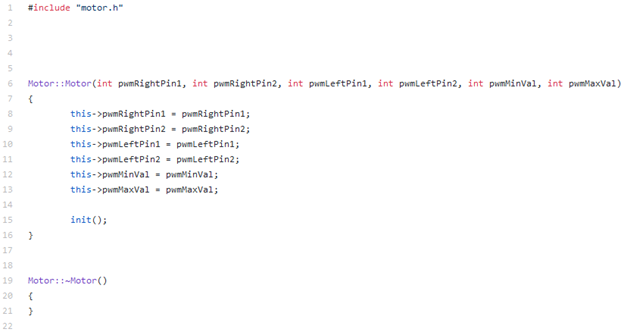
\includegraphics{figures/53.png}
    \caption{Definition Motor Code: motor function}
    \label{fig:my_label}
\end{figure}

\newpage

After that, we define the motion function beginning with the forward function; to make the body go forward we make the right side and the left one go forward as shown in the figure (55) … so we call the functions right Side Forward and left Side Forward. Those functions will be explained later in this code file.

\begin{figure}[h]
  \centering
  \subfloat[Forward function]{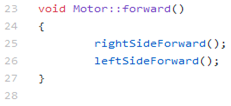
\includegraphics[width=0.5\textwidth]{figures/54.png}\label{fig:f1}}
  \hfill
  \subfloat[Forward Motion]{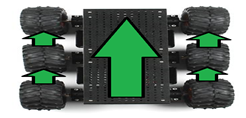
\includegraphics[width=0.5\textwidth]{figures/55.png}\label{fig:f2}}
  \caption{Definition Motor Code: Forward}
\end{figure}

Then, we continue defining the motion function of backward function; to make the body go backward we make the right side and the left one go backward as shown in the figure (57) … so we call the functions right Side Backward and left Side Backward. Those functions will be explained later in this code file.

\begin{figure}[h]
  \centering
  \subfloat[Backward Function]{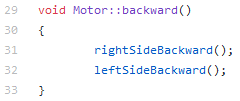
\includegraphics[width=0.5\textwidth]{figures/56.png}\label{fig:f1}}
  \hfill
  \subfloat[Backward Motion]{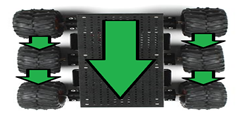
\includegraphics[width=0.5\textwidth]{figures/57.png}\label{fig:f2}}
  \caption{Definition Motor Code: Backward}
\end{figure}

\newpage

Then, we continue defining the motion function of turn Right function; to make the body turn right we make the right side go backward and the left one go forward as shown in the figure (59) … so we call the functions right Side Backward and left Side Forward. Those functions will be explained later in this code file.

\begin{figure}[h]
  \centering
  \subfloat[Turning Right function]{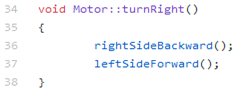
\includegraphics[width=0.5\textwidth]{figures/58.png}\label{fig:f1}}
  \hfill
  \subfloat[Turning Right Motion]{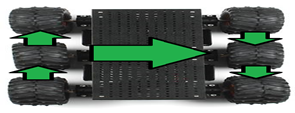
\includegraphics[width=0.5\textwidth]{figures/59.png}\label{fig:f2}}
  \caption{Definition Motor Code: Right}
\end{figure}

Finally, we continue defining the motion function of turn Left function; to make the body turn left we make the right side go forward and the left one go backward as shown in the figure (61) … so we call the functions right Side Forward and left Side Backward. Those functions will be explained later in this code file.

\begin{figure}[h]
  \centering
  \subfloat[Turning Left function]{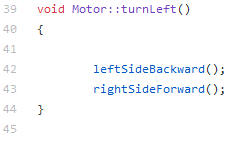
\includegraphics[width=0.5\textwidth]{figures/60.png}\label{fig:f1}}
  \hfill
  \subfloat[Turning Left Motion]{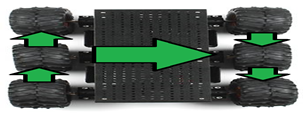
\includegraphics[width=0.5\textwidth]{figures/61.png}\label{fig:f2}}
  \caption{Definition Motor Code: Left}
\end{figure}


After defining the motion function of turn Right function, we define the initialization function. We define the mode of the four PWM pins (Two Left and Two Right) as output pins. Also, we create the voltage range that will be deal with by assign the four pins in ranges of the minimum and maximum PWM values.

\newpage

Note that this initialization is called only when we make an object of motor class; or we can say that the initialization is called one and only at every motor created.  In this code … we have only one motor so this function is called only one time.

\begin{figure}[h]
    \centering
    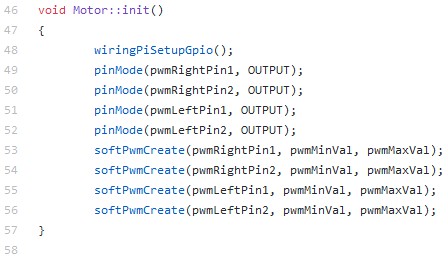
\includegraphics{figures/62.png}
    \caption{Definition Motor Code: init function}
    \label{fig:my_label}
\end{figure}

\newpage
After defining the initialization function, we begin to define the movement of each side forward and backward. We define the movement of Right side forward by assigning high value on Right Pin no. 1 while assigning low value on Right Pin no. 2, Right side backward by assigning low value on Right Pin no. 1 while assigning high value on Right Pin no. 2, Left side forward by assigning high value on Left Pin no. 1 while assigning low value on Left Pin no. 2, and finally Left side Backward by assigning low value on Left Pin no. 1 while assigning high value on Left Pin no.2.

\begin{figure}[h]
\centering
\begin{minipage}{.5\textwidth}
  \centering
  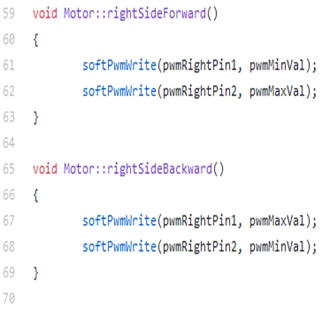
\includegraphics[width=1\linewidth]{figures/63.png}
  \captionof{figure}{Definition Motor Code: Right side functions}
  \label{fig:test1}
\end{minipage}%
\begin{minipage}{.5\textwidth}
  \centering
  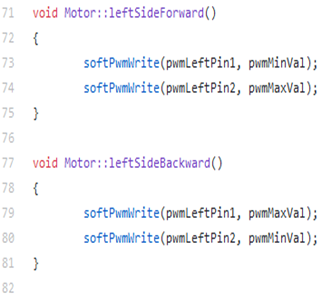
\includegraphics[width=1\linewidth]{figures/64.png}
  \captionof{figure}{Definition Motor Code: Left side functions}
  \label{fig:test2}
\end{minipage}
\end{figure}

\newpage

 After defining the movement of each side forward and backward, we define the stop of the movement of Right side, Left side and the whole body. First we begin with the stop movement of the left side by the same logic of movement the left side but by assigning low value on both Left pins number one and two at stopping left side.

\begin{figure}[h]
    \centering
    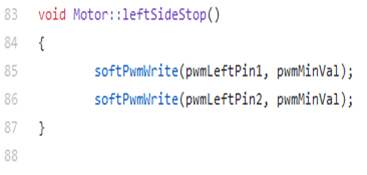
\includegraphics{figures/65.png}
    \caption{Definition Motor Code: Left stop functions}
    \label{fig:my_label}
\end{figure}


Then, we begin with the stop movement of the right side by the same logic of movement the right side but by assigning low value on both right pins number one and two at stopping right side.

\begin{figure}[h]
    \centering
    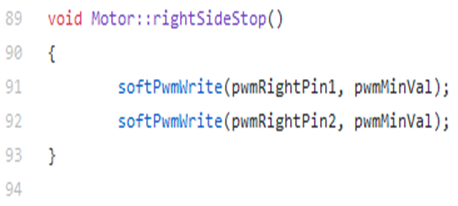
\includegraphics{figures/66.png}
    \caption{Definition Motor Code: Right stop Functions}
    \label{fig:my_label}
\end{figure}

\newpage

Finally, we begin with the stop movement of the whole body by stopping the left and right side from movement by calling the right Side Stop and left Side Stop Functions that where explained before in this code file.

\begin{figure}[h]
    \centering
    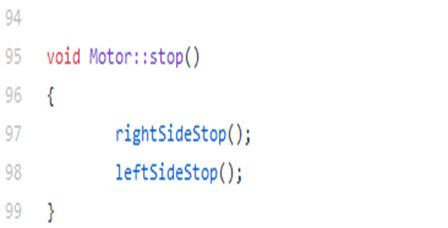
\includegraphics{figures/67.png}
    \caption{Definition Motor Code: Global stop functions}
    \label{fig:my_label}
\end{figure}

\newpage
\subsubsection{The Main Project Code}

This code file named “pro1.cpp” and it is responsible for the main program. In the first, we include the header file which is called ‘motor.h’ that has the declaration of the functions needed to be defined and some other include files we in need for them. In the main block, we create an object from “motor” Class with assigning in it the pin numbers and values required in motor function. We assigned the pins number (20, 21, 13 and 19) as motor pins, assigning ‘0’ for minimum value of PWM value and ‘100’ for maximum value of PWM value. We also declared some variable that will be used including variable named response for the HTTP response, variable named body response for the receiving response status code and, variable named body response for the receiving response status code.

\begin{figure}[h]
    \centering
    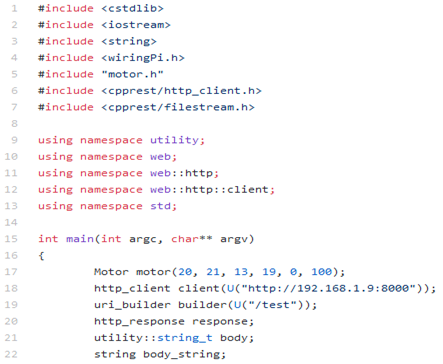
\includegraphics{figures/68.png}
    \caption{Main Project code: Initialization}
    \label{fig:my_label}
\end{figure}

\newpage

In an infinite loop – The program repeated infinite number – we get the Received response status code and assign the value a variable called body that was defined before. If this process doesn’t go well – Any error Occurred – then stop the motor immediately … if the process of getting the code goes good – No error occurred – then do the following code. 

\begin{figure}[h]
    \centering
    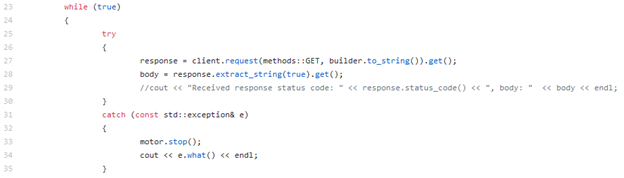
\includegraphics{figures/69.png}
    \caption{Main Project code: Get response status code}
    \label{fig:my_label}
\end{figure}

\newpage

Here, we assign what we get of response status code and check whether the response status code is equal UP then the body move forward, or it is equal DOWN then the body move backward, or it is equal Right then the body turn right, or it is equal LEFT then the body turn left … OR nothing of those condition then the body will stop.

\begin{figure}[h]
    \centering
    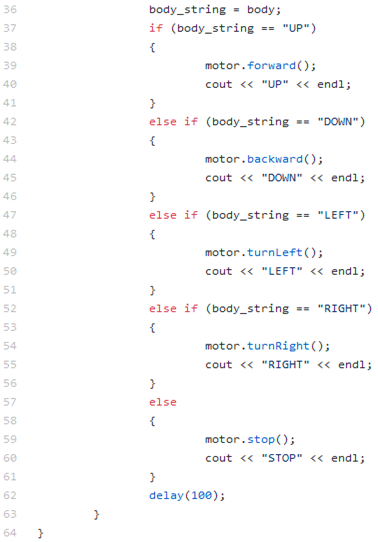
\includegraphics[width=0.6\textwidth]{figures/70.png}
    \caption{Main Project code: Condition block}
    \label{fig:my_label}
\end{figure}
